\documentclass[11pt,a4paper]{article}
\usepackage[utf8]{inputenc}
\usepackage[czech]{babel}
\usepackage[T1]{fontenc}
\usepackage{amsmath}
\usepackage{amsfonts}
\usepackage{amssymb}
\usepackage{graphicx}
\usepackage{enumitem}
\usepackage[includeheadfoot, margin=1in]{geometry}
\usepackage{fancyhdr}
\fancyhf{}
\pagestyle{fancy}
\rhead{Václav Luňák}
\lhead{Domácí úkol na 15. 5. 2018}
\cfoot{\thepage}
\begin{document}
\section*{Příklad 1}
\begin{enumerate}[label=(\alph*)]
\item
Definiční obor funkce $f$ je $\{(x,y) \in R^2 \vert x+y^2 > 0\}$. Tato množina se dá vyjádřit jako $x > -y^2$, což nám dá následující náčrt definičního oboru (okraj do množiny nepatří):\\
\begin{flushright}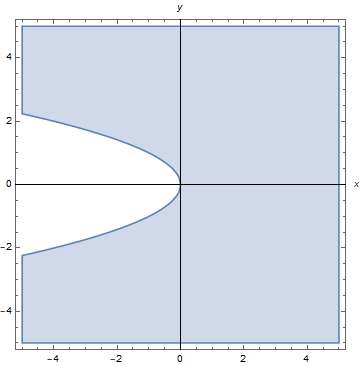
\includegraphics[width=3cm]{09_def.png}\end{flushright}

\item
Nejprve spočteme parciální derivace funkce.
\begin{align*}
\frac{\partial f}{\partial x} = \frac{1}{x+y^2} \\
\frac{\partial f}{\partial y} = \frac{2y}{x+y^2}
\end{align*}
Tyto parciální derivace existují na celém $D$ a jsou všude spojité. Dosazením pak získáme gradient pro bod $[0,1]$
\begin{align*}
\nabla f(0,1) = (1, 2)
\end{align*} 

\item
Funkce má na celém definičním oboru spojité parciální derivace, tedy je všude diferencovatelná.
\begin{align*}
	& Df_{(1,1)}(x,y) = \frac{1}{1+1^y}(x-1)+\frac{2\cdot 1}{1+1^2}(y-1) = \frac{x-1}{2} + (y-1)
\end{align*}

\item
\begin{align*}
	& Df_{(0,1)}(x,y) = x+2(y-1)\\
	& Df_{(0,1)}(0.04,0.99) = 0.02\\
	& f(0.04,0.99) \approx f(0,1) + Df_{(0,1)}(0.04,0.99) = 0 + 0.02 = 0.02 
\end{align*}

\item
\begin{align*}
	& \tau : z = x + 2(y-1) + 0 \Rightarrow x + 2y - z - 2 = 0
\end{align*}
\end{enumerate}

\section*{Příklad 2}
\begin{align*}
	& L = \sqrt{3}x-y+2 -\lambda(x^2 + 2x + y^2) \\
	& \frac{\partial L}{\partial x} = \sqrt{3} - 2\lambda x -2\lambda = 0 \\
	& \frac{\partial L}{\partial y} = -1 - 2\lambda y  = 0\\
	& x^2 + 2x + y^2 = 0	
\end{align*}
Tato soustava nám dává dvě řešení: $a = (-1-\frac{\sqrt{3}}{2}, \frac{1}{2})$ a $b = (-1+\frac{\sqrt{3}}{2}, -\frac{1}{2})$. Zbývá nám prozkoumat body, ve kterých je nulový gradient $f$.

\begin{align*}
	& \frac{\partial f}{\partial x} = \sqrt{3}
	& \frac{\partial f}{\partial y} = -1
\end{align*}
Jelikož $f$ má vždy nenulový gradient a $M$ je kompaktní, musí body ze soustavy být extrémy. Po dosazení získáváme, že $b$ je maximum a $a$ minimum. 
\end{document}